\documentclass[a4paper,12pt]{article}

% Codificación y lenguaje
\usepackage[utf8]{inputenc}
\usepackage[T1]{fontenc}
\usepackage[spanish]{babel}
\usepackage[utf8]{inputenc}

% Paquetes esenciales
\usepackage{graphicx}
\usepackage{geometry}
\usepackage{datetime}
\usepackage{titlesec}
\usepackage{fancyhdr}
\usepackage{parskip}
\usepackage{array}
\usepackage{float}
\usepackage{placeins}
\usepackage{hyperref}
% Paquetes para código fuente
\usepackage{listings}
\usepackage{xcolor}
\usepackage{amsmath}  

% Configuración del estilo de listings para código Arduino
\lstdefinestyle{arduino}{
  language=C++,
  basicstyle=\ttfamily\footnotesize,
  keywordstyle=\color{blue},
  commentstyle=\color{gray},
  stringstyle=\color{red},
  numbers=left,
  numberstyle=\tiny,
  stepnumber=1,
  numbersep=5pt,
  backgroundcolor=\color{white},
  frame=single,
  breaklines=true,
  captionpos=b
}
\lstset{style=arduino}

% Márgenes del documento
\geometry{left=3cm, right=2.5cm, top=3cm, bottom=3cm}

\begin{document}

\begin{titlepage}
    \begin{center}
        {\LARGE \textbf{Universidad Nacional de Córdoba}}\\[1.5cm]

        
\includegraphics[scale=0.4]{img/logo2.png}\\[1.5cm]

        {\large Facultad de Ciencias Exactas, Físicas y Naturales}\\

        \rule{\linewidth}{0.5mm}\\[0.4cm]
        {\Large \textbf{Cátedra de Arquitectura de Computadoras}}\\[0.3cm]
        {\LARGE \textbf{Trabajo Práctico 1: ALU}}\\[0.3cm]
        \rule{\linewidth}{0.5mm}\\[1cm]

        \begin{flushleft}
        {\large 
            \textbf{Profesores:} - Martin Pereyra, Santiago Rodriguez\\
            \textbf{Integrantes:}\\
            Pallardó Agustín - 
            \href{mailto:apallardo@mi.unc.edu.ar}{apallardo@mi.unc.edu.ar}\\
            Trachta Agustín - 
            \href{mailto:agutrachta@mi.unc.edu.ar}{agutrachta@mi.unc.edu.ar}\\
        }
        \end{flushleft}

        \vfill

        {\large \today}
    \end{center}
\end{titlepage}
\tableofcontents
\clearpage
\section{Introducción}

La comunicación serie es uno de los mecanismos más utilizados en sistemas digitales para transmitir información de manera simple y eficiente. Dentro de este esquema, el estándar \textbf{UART} (Universal Asynchronous Receiver/Transmitter) constituye una de las soluciones más difundidas debido a su simplicidad de implementación, bajo costo y compatibilidad con una amplia variedad de dispositivos.

En este trabajo se presenta el diseño e implementación de un sistema digital basado en \textbf{UART}, desarrollado en lenguaje \textit{Verilog HDL}. El sistema no solo incluye los bloques clásicos de transmisión y recepción, sino que además incorpora:

\begin{itemize}
    \item \textbf{Un generador de baudios} para sincronizar la comunicación.
    \item \textbf{Memorias FIFO} que permiten desacoplar los datos recibidos y transmitidos.
    \item \textbf{Una Unidad Aritmético-Lógica (ALU)} encargada de procesar los operandos recibidos.
    \item \textbf{Un bloque de interfaz} que organiza los datos provenientes del canal serie para dirigirlos a la ALU y reenviar los resultados.
\end{itemize}

El objetivo principal es demostrar cómo la arquitectura UART puede extenderse más allá de la simple comunicación, integrándose con módulos de procesamiento para construir sistemas digitales completos. En particular, se busca implementar un mecanismo mediante el cual se reciben instrucciones desde un puerto serie, se procesan mediante la ALU y los resultados se reenvían nuevamente al transmisor UART.

El trabajo se organiza de la siguiente manera: primero se describen los módulos fundamentales en orden de ejecución (generador de baudios, receptor, FIFO, transmisor, ALU e interfaz). Posteriormente, se analiza la integración en el módulo \texttt{top}, se presentan las simulaciones y pruebas realizadas, y finalmente se discuten los resultados obtenidos junto con posibles mejoras.

\clearpage
\section{Descripción general del sistema}

El diseño implementado corresponde a un sistema UART extendido con capacidades de procesamiento mediante una \textbf{Unidad Aritmético-Lógica (ALU)}. El bloque superior \texttt{top} integra todos los módulos que lo componen y define el flujo de datos completo desde la entrada serie (\texttt{rx}) hasta la salida (\texttt{tx}).

\subsection{Bloque \texttt{top}}
El módulo \texttt{top} actúa como entidad principal, interconectando:
\begin{itemize}
    \item El generador de baudios, encargado de derivar la señal de muestreo \texttt{sample\_tick}.
    \item El receptor UART (\texttt{uart\_rx}), que reconstruye bytes a partir de la señal serie entrante.
    \item Dos memorias FIFO: una para los datos recibidos y otra para los datos a transmitir.
    \item El transmisor UART (\texttt{uart\_tx}), que serializa los datos de salida.
    \item El módulo \texttt{interface}, encargado de interpretar los bytes recibidos como operación y operandos, y enviar los resultados a la FIFO de transmisión.
    \item La ALU, que realiza las operaciones aritméticas y lógicas definidas.
\end{itemize}

\subsection{Esquemático general}
La Figura~\ref{fig:uart-general} muestra un diagrama de bloques típico de un sistema UART completo, donde se observa la integración del generador de baudios, los bloques de transmisión y recepción, y las memorias FIFO.

\begin{figure}[H]
    \centering
    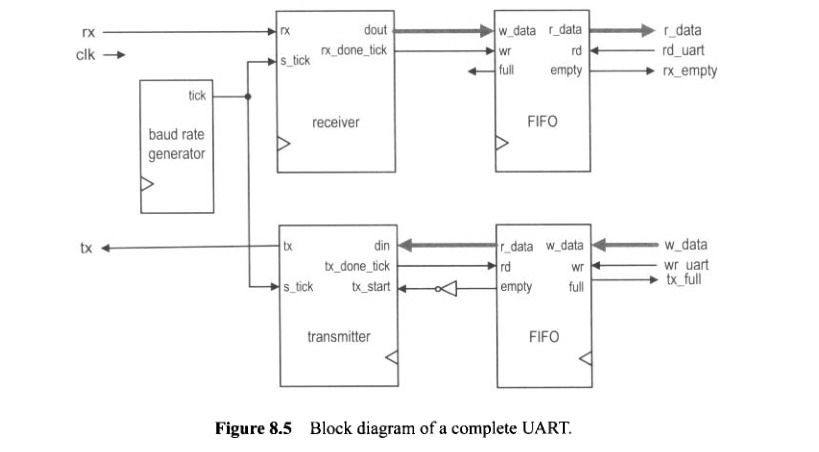
\includegraphics[width=0.75\textwidth]{img/completeUART.jpeg}
    \caption{Diagrama de bloques de un UART completo \cite{libroUART}.}
    \label{fig:uart-general}
\end{figure}

\subsection{Flujo de datos}
El flujo de información en el sistema sigue la siguiente secuencia:
\begin{enumerate}
    \item Los datos ingresan por la línea \texttt{rx} y son muestreados por el \texttt{uart\_rx}.
    \item Los bytes reconstruidos se almacenan en la \textbf{FIFO RX}.
    \item El módulo \texttt{interface} extrae los datos de la FIFO y organiza los tres bytes requeridos: código de operación, operando A y operando B.
    \item La ALU procesa estos valores y genera un resultado.
    \item El resultado se escribe en la \textbf{FIFO TX}.
    \item Finalmente, el \texttt{uart\_tx} serializa el dato y lo envía por la línea \texttt{tx}.
\end{enumerate}

\clearpage
\section{Generador de baudios (\texttt{baud\_gen})}

El primer bloque del sistema es el generador de baudios, cuya función es producir la señal de muestreo necesaria para sincronizar tanto la recepción como la transmisión de datos. 

\subsection{Principio de funcionamiento}
El módulo recibe como entradas el reloj principal de la FPGA (\texttt{clk}) y la señal de \texttt{reset}. 
A partir de un divisor interno, genera una señal periódica llamada \texttt{sample\_tick}, que es utilizada por los módulos \texttt{uart\_rx} y \texttt{uart\_tx} para sincronizar sus máquinas de estados.

El cálculo del divisor se realiza en función de la frecuencia de reloj de la FPGA y de la tasa de baudios deseada:
\[
DIVISOR = \frac{f_{clk}}{BAUD\_RATE \times 16}
\]
donde el factor 16 corresponde al \textit{oversampling}, una técnica habitual en UART que permite mejorar la detección de bits y reducir errores por jitter o pequeñas diferencias de frecuencia.

\subsection{Oversampling en UART}

En UART asíncrono el emisor y el receptor no comparten reloj, por lo que el receptor debe \emph{reconstruir} el instante de muestreo de cada bit a partir del flanco del \emph{start bit}. Para mejorar la robustez frente a pequeñas desintonías de baudios, jitter y ruido, se utiliza \textbf{oversampling}: muestrear cada bit varias veces a una frecuencia $M$ veces superior a la tasa de baudios.

En este diseño se emplea $M=16$, por lo que el generador de baudios produce una señal de \emph{tick} con:
\[
f_{\text{tick}} = M \cdot BAUD\_RATE \qquad \Rightarrow \qquad T_{\text{tick}} = \frac{T_{\text{bit}}}{M}
\]
El receptor detecta el flanco descendente del start, espera \(\tfrac{M}{2}\) ticks (centro del start) y a partir de allí toma una muestra cada \(M\) ticks, que caen en el \textbf{centro} de cada bit de datos. Muestrear en el centro maximiza el margen a distorsiones temporales.

\subsection{Flujo interno}
\begin{itemize}
    \item Un contador se incrementa en cada flanco ascendente del reloj principal.
    \item Cuando el contador alcanza el valor del divisor, se reinicia y se genera un pulso en \texttt{sample\_tick}.
    \item Este pulso marca los instantes exactos en que deben muestrearse o transmitirse los bits.
\end{itemize}

\subsection{Importancia en el sistema}
El \texttt{baud\_gen} es esencial porque garantiza que tanto el transmisor como el receptor trabajen bajo la misma temporización. 
En caso contrario, existiría desalineación entre los bits enviados y los recibidos, ocasionando errores en la reconstrucción de los datos.  
Gracias a su parametrización, este módulo es flexible y puede adaptarse fácilmente a distintas frecuencias de reloj y diferentes tasas de transmisión.

\clearpage
\section{Receptor UART (\texttt{uart\_rx})}

El receptor es responsable de transformar la señal serie \texttt{rx} en un byte paralelo y anunciar cuándo el dato está listo. Emplea \textbf{oversampling} a $16\times$ y una máquina de estados finitos (FSM) con temporización por ticks.

\subsection{Trama y convenciones}
La línea \texttt{rx} permanece en nivel alto en reposo. Cada trama se compone de:
\begin{itemize}
    \item \textbf{Start}: 1 bit en nivel bajo.
    \item \textbf{Datos}: \(\texttt{DBIT}=8\) bits, orden \textit{LSB first}.
    \item \textbf{Stop}: 1, 1.5 o 2 bits en alto, parametrizados por \(\texttt{SB\_TICK}\in\{16,24,32\}\).
\end{itemize}

\subsection{Señales y contadores internos}
\begin{itemize}
    \item \texttt{sample\_tick}: pulso de temporización a \(16\times\) la tasa de baudios.
    \item \texttt{tick\_count}: cuenta los ticks dentro del bit (0..15 para datos).
    \item \texttt{bit\_count}: cuenta cuántos bits de datos se han muestreado (0..DBIT-1).
    \item \texttt{rx\_shift\_reg}: registro de desplazamiento donde se van incorporando los bits recibidos.
    \item \texttt{rx\_done\_tick}: pulso de un ciclo de \texttt{clk} que indica “byte listo”.
\end{itemize}

\subsection{Máquina de estados y flujo temporal}
La FSM consta de cuatro estados: \textbf{IDLE}, \textbf{START}, \textbf{DATA} y \textbf{STOP}. El funcionamiento se describe paso a paso a continuación y se ilustra en la Figura~\ref{fig:uart-rx-fsm}.

\paragraph{1) IDLE (espera de start)}  
La línea \texttt{rx} está alta. Al detectarse un nivel bajo (\emph{start bit}), se pasa a \textbf{START} y se reinicia \texttt{tick\_count}.

\paragraph{2) START (centrado de muestreo)}  
Con cada \texttt{sample\_tick} se incrementa \texttt{tick\_count}. Al alcanzar \(\texttt{tick\_count}=7\) (8 ticks desde el flanco), se considera que estamos en el \textbf{centro} del start. Entonces:
\begin{enumerate}
    \item Se pone \texttt{tick\_count} en 0 para comenzar a cronometrar el primer bit de datos.
    \item Se pone \texttt{bit\_count} en 0.
    \item Se transita a \textbf{DATA}.
\end{enumerate}

\paragraph{3) DATA (muestreo de 8 bits)}  
Cada vez que \(\texttt{tick\_count}=15\) y llega \texttt{sample\_tick}, se toma la muestra del bit (centro del bit) y se la introduce al MSB del \texttt{rx\_shift\_reg} desplazando a la derecha. Esto, repetido 8 veces con \textit{LSB first}, deja el registro en orden natural \([b7\ldots b0]\). Tras cada muestreo:
\begin{itemize}
    \item \texttt{tick\_count} se reinicia a 0.
    \item \texttt{bit\_count} se incrementa.  
          Si \(\texttt{bit\_count}= \texttt{DBIT}-1\), se pasa a \textbf{STOP}.
\end{itemize}

\paragraph{4) STOP (validación y fin de trama)}  
Se esperan \(\texttt{SB\_TICK}\) ticks (por defecto 16 para 1 bit de stop). Al cumplirse:
\begin{itemize}
    \item Se genera un pulso \texttt{rx\_done\_tick} indicando que el byte en \texttt{dout} es válido.
    \item Se vuelve a \textbf{IDLE}.
\end{itemize}

\begin{figure}[H]
    \centering
    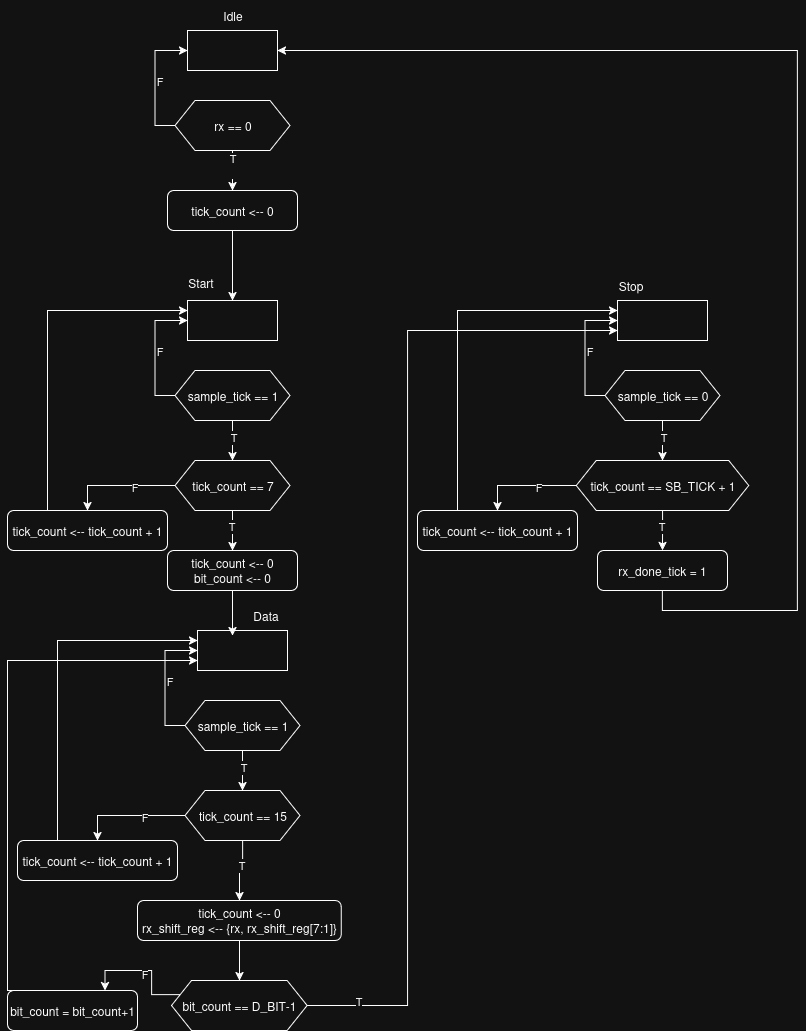
\includegraphics[width=0.95\textwidth]{img/diagramaReceiverUART.png}
    \caption{Diagrama de flujo de la FSM del receptor UART con oversampling a \(16\times\).}
    \label{fig:uart-rx-fsm}
\end{figure}

\subsection{Cronometría: instantes de muestreo}
Tras detectar el start, el primer muestreo útil ocurre \(8\) ticks después (centro del start) y luego cada \(16\) ticks para cada bit de datos. El tiempo total entre el flanco de start y el anuncio del byte listo es:
\[
N_{\text{ticks}} = 8 + 16\cdot \texttt{DBIT} + \texttt{SB\_TICK}
\]
Para \(\texttt{DBIT}=8\) y \(\texttt{SB\_TICK}=16\): \(N_{\text{ticks}}=152\).  
Como \(T_{\text{tick}}=\tfrac{1}{16\cdot BAUD\_RATE}\), el retardo es aproximadamente \(152 \cdot T_{\text{tick}} \approx 0{,}99\,\text{ms}\) a \(9600\,\text{bps}\), coherente con una trama de 10 bits (\(\sim 1{,}04\,\text{ms}\)), considerando que el muestreo se inicia en el centro del start.

\subsection{Parámetros y salidas}
\begin{itemize}
    \item \textbf{\texttt{DBIT}}: número de bits de datos (8 en este diseño).
    \item \textbf{\texttt{SB\_TICK}}: cantidad de ticks de stop (16, 24 o 32 $\Rightarrow$ 1, 1.5 o 2 bits).
    \item \textbf{\texttt{dout}}: byte paralelo reconstruido a partir de \texttt{rx\_shift\_reg}.
    \item \textbf{\texttt{rx\_done\_tick}}: pulso de 1 ciclo de \texttt{clk} indicando dato válido.
\end{itemize}

\subsection{Notas de diseño y posibles mejoras}
\begin{itemize}
    \item \textbf{Sincronización del pin \texttt{rx}}: al ser asíncrono respecto de \texttt{clk}, es recomendable anteponer un \emph{doble flip-flop} de sincronización para mitigar metastabilidad.
    \item \textbf{Detección de error de trama}: durante \textbf{STOP} verificar que \texttt{rx} esté alto; si no, reportar \emph{framing error}.
\end{itemize}

\clearpage
\section{Transmisor UART (\texttt{uart\_tx})}

El bloque \texttt{uart\_tx} es el encargado de serializar un dato paralelo de 8 bits y enviarlo a través de la línea \texttt{tx}, siguiendo la convención de trama UART: un bit de inicio, 8 bits de datos y un bit de parada (o más, según configuración).

\subsection{Principio de funcionamiento}
El transmisor se activa cuando recibe la señal \texttt{tx\_start}, lo que indica que existe un byte válido en su registro de entrada (\texttt{din}). A partir de ese momento, controla la línea \texttt{tx} mediante una máquina de estados finitos (FSM) que sigue la misma temporización definida por los pulsos de \texttt{sample\_tick} generados por el módulo \texttt{baud\_gen}.

\subsection{Máquina de estados}
El transmisor implementa los mismos cuatro estados que el receptor:
\begin{itemize}
    \item \textbf{IDLE}: la línea \texttt{tx} permanece en nivel alto. Espera que la señal \texttt{tx\_start} se active.
    \item \textbf{START}: coloca la línea en nivel bajo durante 16 ticks para indicar el comienzo de la trama.
    \item \textbf{DATA}: envía uno a uno los bits de datos, en orden \textit{LSB first}. Cada bit permanece estable durante 16 ticks.
    \item \textbf{STOP}: fuerza la línea a nivel alto durante \texttt{SB\_TICK} ticks. Una vez cumplido, emite el pulso \texttt{tx\_done\_tick} y vuelve a \textbf{IDLE}.
\end{itemize}

\subsection{Flujo interno}
El dato a transmitir se carga en un registro de desplazamiento (\texttt{tx\_shift\_reg}) cuando \texttt{tx\_start} se activa.  
En cada ciclo de envío de bit:
\begin{itemize}
    \item El bit menos significativo del registro se coloca en la línea \texttt{tx}.
    \item Al completarse los 16 ticks, el registro se desplaza a la derecha para preparar el siguiente bit.
\end{itemize}

\subsection{Comparación con el receptor}
El \texttt{uart\_tx} utiliza la misma estructura general que el receptor:
\begin{itemize}
    \item Ambos cuentan con una FSM con los estados \textbf{IDLE}, \textbf{START}, \textbf{DATA} y \textbf{STOP}.
    \item Ambos utilizan los pulsos de \texttt{sample\_tick} para sincronizar los instantes de transmisión o muestreo.
\end{itemize}

Las diferencias clave son:
\begin{itemize}
    \item El receptor \texttt{uart\_rx} reconstruye bits desde la línea serie hacia un registro, mientras que el transmisor hace el proceso inverso: toma un byte paralelo y lo serializa.
    \item El transmisor siempre conoce los tiempos exactos en los que debe cambiar el valor de la línea, mientras que el receptor debe detectar el inicio de la trama y re-alinearse a partir de allí.
\end{itemize}

\subsection{Señales principales}
\begin{itemize}
    \item \textbf{\texttt{din}}: dato paralelo de entrada (8 bits).
    \item \textbf{\texttt{tx}}: línea de transmisión serie.
    \item \textbf{\texttt{tx\_start}}: pulso que indica al transmisor que debe enviar el byte cargado.
    \item \textbf{\texttt{tx\_done\_tick}}: pulso de un ciclo de \texttt{clk} que indica que la transmisión finalizó.
\end{itemize}

\clearpage
\section{Memoria FIFO (\texttt{fifo})}

La FIFO (First-In, First-Out) es el bloque que \textbf{desacopla} temporalmente los productores y consumidores de datos. En este proyecto se utilizan dos, como vimos en la figura~\ref{fig:uart-general}: una a la salida del receptor (\textbf{FIFO RX}) y otra a la entrada del transmisor (\textbf{FIFO TX}). Su función es absorber ráfagas y tolerar pequeñas desincronizaciones entre módulos.

\begin{figure}[H]
    \centering
    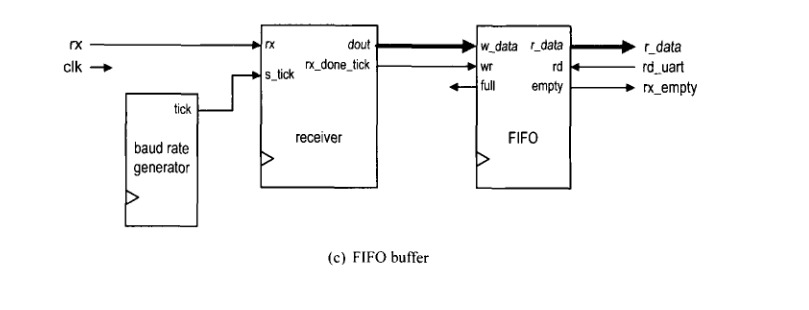
\includegraphics[width=0.78\textwidth]{img/FIFObuffer.jpeg}
    \caption{Inserción de una FIFO a la salida del receptor UART.}
    \label{fig:fifo-buffer}
\end{figure}

\subsection{Estructura y señales}
La FIFO es \textbf{sincronizada a un único reloj} (\texttt{clk}) y parametrizable:
\begin{itemize}
    \item \textbf{Ancho de palabra} \(W\) (bits por elemento).
    \item \textbf{Profundidad} \(N\) (cantidad de elementos).
\end{itemize}

Interfaz:
\begin{itemize}
    \item \texttt{w\_data} (entrada de datos), \texttt{wr} (pedido de escritura) y \texttt{full} (FIFO llena).
    \item \texttt{r\_data} (salida de datos), \texttt{rd} (pedido de lectura) y \texttt{empty} (FIFO vacía).
\end{itemize}

\subsection{Punteros y contador}
Internamente mantiene:
\begin{itemize}
    \item \textbf{Puntero de escritura} \(w\_ptr\) y \textbf{puntero de lectura} \(r\_ptr\), ambos de ancho \(\lceil \log_2 N \rceil\). Al incrementarse, \textbf{envolvieron} (wrap-around) de manera circular.
    \item \textbf{Contador de ocupación} \(count\) en el rango \(0 \ldots N\). De él se derivan las banderas:
    \[
        \texttt{empty} \Leftrightarrow count=0,\qquad
        \texttt{full}  \Leftrightarrow count=N.
    \]
\end{itemize}

\textbf{Nota de diseño:} si \(N\) \emph{no} es potencia de 2, conviene implementar un \emph{wrap} explícito (\(w\_ptr \leftarrow 0\) cuando \(w\_ptr=N-1\), idem \(r\_ptr\)) para garantizar que nunca se indexe fuera de \(0 \ldots N-1\).

\subsection{Escritura y lectura}
\paragraph{Escritura (lado productor).}
En el flanco ascendente de \texttt{clk}, si \texttt{wr} está activo y la FIFO \textbf{no} está llena, se copia \texttt{w\_data} en la posición indicada por \(w\_ptr\) y luego:
\[
w\_ptr \leftarrow w\_ptr + 1,\quad count \leftarrow count + 1.
\]

\paragraph{Lectura (lado consumidor).}
La salida \texttt{r\_data} refleja el contenido de la posición apuntada por \(r\_ptr\) (\emph{estilo FWFT, first-word fall-through}). Cuando el consumidor afirma \texttt{rd} y la FIFO \textbf{no} está vacía, en el próximo flanco:
\[
r\_ptr \leftarrow r\_ptr + 1,\quad count \leftarrow count - 1.
\]
Esto “avanza” la ventana y el siguiente dato queda disponible de inmediato en \texttt{r\_data} tras ese flanco.

\subsection{Lectura y escritura simultáneas}
Si en un mismo ciclo se cumple \(\texttt{wr}\wedge\neg\texttt{full}\) \emph{y} \(\texttt{rd}\wedge\neg\texttt{empty}\):
\[
w\_ptr \leftarrow w\_ptr + 1,\qquad r\_ptr \leftarrow r\_ptr + 1,\qquad count \text{ no cambia}.
\]
La ocupación permanece constante, lo que permite \textbf{canalizar} (pipeline) productor y consumidor sin bloqueo.

\subsection{Reset y mapeo en hardware}

Cuando se activa la señal de \texttt{reset}, la FIFO vuelve a su estado inicial:
\begin{itemize}
    \item Los punteros de lectura y escritura se ponen en cero.
    \item El contador de ocupación también se pone en cero.
\end{itemize}

Esto asegura que la memoria comience \textbf{vacía}.  

\subsection{Manejo correcto del \emph{handshake}}
\begin{itemize}
    \item El \textbf{productor} debe escribir solo cuando \(\neg\texttt{full}\).
    \item El \textbf{consumidor} debe leer solo cuando \(\neg\texttt{empty}\).
    \item Las banderas \texttt{full}/\texttt{empty} evitan \emph{overflow/underflow}.
\end{itemize}

\subsection*{Uso en el receptor (FIFO RX)}
A la salida del \texttt{uart\_rx}, cada vez que se completa una trama se genera \texttt{rx\_done\_tick}; ese pulso se utiliza como \texttt{wr} de la FIFO RX y el byte recibido ingresa como \texttt{w\_data}.  
El bloque \texttt{interface} actúa como \textbf{consumidor}: monitorea \texttt{empty}; cuando hay datos, aserta \texttt{rd} (señal \texttt{rd\_uart} en el diseño) para avanzar y tomar el próximo byte en \texttt{r\_data}. Así, el receptor puede seguir capturando tramas aunque el procesamiento sea más lento.

\subsection*{Uso en el transmisor (FIFO TX)}
La \texttt{interface} escribe en la FIFO TX el \textbf{resultado} de la ALU (\texttt{wr\_uart} como \texttt{wr}), siempre que \(\neg\texttt{full}\).  
El \texttt{uart\_tx} es el \textbf{consumidor}: cuando termina de enviar un byte, aserta \texttt{tx\_done\_tick} que hace de \texttt{rd} para tomar automáticamente el siguiente. En el \texttt{top}, la señal \texttt{tx\_start} se activa mientras la FIFO TX \textbf{no} esté vacía (\(\texttt{tx\_start} \leftarrow \neg \texttt{tx\_empty}\)), logrando una transmisión continua si hay datos en cola.

\clearpage
\section{Unidad Aritmético-Lógica (ALU)}

La ALU es el bloque encargado de realizar operaciones aritméticas y lógicas sobre dos operandos de 8 bits.  
Se controla mediante un código de operación de 6 bits que determina qué función ejecutar.  

\subsection{Operaciones soportadas}
\begin{table}[H]
    \centering
    \begin{tabular}{|c|c|c|}
        \hline
        Código (binario) & Operación & Descripción \\ \hline
        100000 & ADD & Suma de \texttt{A + B} \\
        100010 & SUB & Resta \texttt{A - B} \\
        100100 & AND & AND bit a bit \\
        100101 & OR  & OR bit a bit \\
        100110 & XOR & XOR bit a bit \\
        000011 & SRA & Desplazamiento aritmético a derecha \\
        000010 & SRL & Desplazamiento lógico a derecha \\
        100111 & NOR & NOR bit a bit \\ \hline
    \end{tabular}
    \caption{Operaciones soportadas por la ALU.}
    \label{tab:alu-ops}
\end{table}

\subsection{Rol en el sistema}
La ALU recibe como entradas dos datos (\texttt{data\_a}, \texttt{data\_b}) y un código de operación (\texttt{op}), generando un resultado de 8 bits que se almacena en la FIFO de transmisión.  
Esto permite extender la comunicación UART más allá de la simple transferencia de bytes, agregando capacidad de procesamiento en hardware.

\clearpage
\section{Interfaz, decoder y regfile}

\subsection{Máquina de estados de la interfaz}

La interfaz se rediseñó para recibir cuatro bytes por UART, ensamblar una instrucción de 32~bits y despachar su ejecución a través del \textit{decoder}, el \textit{regfile} y la ALU. La FSM emplea los siguientes estados:

\begin{verbatim}
localparam S_IDLE = 3'd0,
           S_I0   = 3'd1,
           S_I1   = 3'd2,
           S_I2   = 3'd3,
           S_I3   = 3'd4,
           S_EX   = 3'd5,
           S_WB   = 3'd6,
           S_TX   = 3'd7;
\end{verbatim}


\begin{itemize}
    \item \textbf{S\_IDLE (reposo).} Estado de espera tras \textit{reset}. Si la bandera de FIFO RX indica disponibilidad de dato (\texttt{\textasciitilde rx\_empty}), se inicia la secuencia de lectura y se transita a \textbf{S\_I0}.
    \item \textbf{S\_I0, S\_I1, S\_I2 (fetch de bytes 0--2).} En cada uno de estos estados, cuando hay dato válido en FIFO RX y se aserta \texttt{rd\_uart}, se lee un byte y se almacena en el \textit{slice} correspondiente de la instrucción (LSB primero). Cada estado avanza al siguiente: \textbf{S\_I0}→\textbf{S\_I1}→\textbf{S\_I2}.
    \item \textbf{S\_I3 (fetch del byte 3).} Se captura el cuarto byte (MSB) y, con la instrucción completa (\(\texttt{instr}[31{:}0]\)), se avanza a \textbf{S\_EX} para ejecutar.
    \item \textbf{S\_EX (ejecución).} Se habilita el flujo hacia el \textit{decoder} para clasificar la instrucción y obtener campos (\texttt{rd}, \texttt{rs1}, \texttt{rs2}, \texttt{imm}) y el selector \texttt{alu\_op}. Con esta información, la interfaz coordina la lectura de operandos del \textit{regfile} y presenta \texttt{alu\_a}, \texttt{alu\_b} y \texttt{alu\_op} a la ALU. El estado siguiente es \textbf{S\_WB}.
    \item \textbf{S\_WB (write-back).} Una vez estable el resultado de la ALU, si la instrucción es de tipo R/I y el destino es distinto de \(x0\), se habilita la escritura del \textit{regfile} (\texttt{we}, \texttt{waddr}=\texttt{rd}, \texttt{wdata}=\texttt{alu\_result}). Luego se transita a \textbf{S\_TX}.
    \item \textbf{S\_TX (respuesta).} Si la FIFO de transmisión (\textbf{FIFO TX}) no está llena, se inserta un byte de respuesta (\texttt{w\_data}, típicamente \(\texttt{alu\_result}[7{:}0]\)) mediante un pulso \texttt{wr\_uart}. Concluida la inserción, la FSM retorna a \textbf{S\_IDLE}.
\end{itemize}

\newpage

\subsection{Bloque secuencial de ensamblado de instrucción}

El ensamblado de la palabra de 32~bits se realiza LSB\(\rightarrow\)MSB, tal como se indica:

\begin{verbatim}
case (state)
  S_I0: if (!rx_empty && rd_uart) instr[7:0]   <= r_data;   // byte 0 (LSB)
  S_I1: if (!rx_empty && rd_uart) instr[15:8]  <= r_data;   // byte 1
  S_I2: if (!rx_empty && rd_uart) instr[23:16] <= r_data;   // byte 2
  S_I3: if (!rx_empty && rd_uart) instr[31:24] <= r_data;   // byte 3 (MSB)
  default: ;
endcase
\end{verbatim}

Un segundo bloque secuencial independiente actualiza el registro de estado (\texttt{state}) con \texttt{state\_n} en el flanco de reloj, desacoplando la lógica combinacional de siguiente estado del almacenamiento sincrónico.

\subsection{Decodificación de la instrucción}

El \textit{decoder} clasifica la instrucción observando \texttt{opcode}/\texttt{funct3}/\texttt{funct7} y expone:
\begin{itemize}
  \item Formato: \(\texttt{is\_rtype}\) (registro--registro) o \(\texttt{is\_itype}\) (registro--inmediato).
  \item Campos: \(\texttt{rd}\), \(\texttt{rs1}\), \(\texttt{rs2}\); e \(\texttt{imm\_i}\) (signado) para tipo I.
  \item Selector de operación de ALU: \(\texttt{alu\_op}\).
\end{itemize}
En particular, si \(\texttt{opcode} = \texttt{7'b0110011}\) la instrucción es \textbf{tipo R} (ALU reg--reg), y si \(\texttt{opcode} = \texttt{7'b0010011}\) es \textbf{tipo I} (ALU reg--imm). El \textit{decoder} no ejecuta; únicamente clasifica y provee los campos para la etapa de ejecución.

\subsection{Camino de datos: \textit{regfile}, ALU y respuesta}

Con los campos del \textit{decoder}, la interfaz direcciona el \textit{regfile} para leer operandos:
\begin{itemize}
  \item Tipo R: \(\texttt{alu\_a} \leftarrow \texttt{rdata\_a}(\texttt{rs1})\), \(\texttt{alu\_b} \leftarrow \texttt{rdata\_b}(\texttt{rs2})\).
  \item Tipo I: \(\texttt{alu\_a} \leftarrow \texttt{rdata\_a}(\texttt{rs1})\), \(\texttt{alu\_b} \leftarrow \texttt{imm\_i}\) (ajustado al ancho de dato).
\end{itemize}
La ALU computa el resultado en función de \(\texttt{alu\_op}\). En \textbf{S\_WB}, si \(\texttt{rd}\neq 0\) y la instrucción es R/I, la interfaz habilita la escritura del \textit{regfile} con \(\texttt{alu\_result}\). En \textbf{S\_TX}, la interfaz inserta en FIFO TX un byte de respuesta (si el protocolo lo requiere) y retorna a \textbf{S\_IDLE}.

\newpage

\subsection{Observaciones de diseño}

\begin{itemize}
  \item La política LSB\(\rightarrow\)MSB en el ensamblado asegura compatibilidad con el flujo de bytes UART.
  \item Es recomendable registrar \(\texttt{alu\_result}\) al final de \textbf{S\_EX} para garantizar estabilidad temporal en \textbf{S\_WB}/\textbf{S\_TX}.
  \item Como mejora futura, puede añadirse un temporizador de \emph{timeout} durante \textbf{S\_I0}--\textbf{S\_I3} para descartar instrucciones incompletas, junto con un mecanismo básico de verificación de integridad.
\end{itemize}

\end{document}